% fig5-sheaf-analysis.tex
% Sheaf Analysis: Goal Equivalence and Tactic Transformations
\documentclass[tikz,border=5pt]{standalone}

% common-styles.tex
% Shared TikZ styles for wonton-proof paper figures

\usepackage{silence}
\WarningFilter{latex}{Missing character} 
\tracinglostchars=0 % Suppress engine-level "Missing character" warnings

\usepackage{fontspec}
\usepackage{unicode-math}

% Use filenames for reliability with Tectonic
\setmainfont{LibertinusSerif-Regular.otf}[
    BoldFont=LibertinusSerif-Bold.otf,
    ItalicFont=LibertinusSerif-Italic.otf,
    BoldItalicFont=LibertinusSerif-BoldItalic.otf
]
\setsansfont{LibertinusSans-Regular.otf}[
    BoldFont=LibertinusSans-Bold.otf,
    ItalicFont=LibertinusSans-Italic.otf
]
\setmonofont{LibertinusMono-Regular.otf}

% Try a more standard math font if LibertinusMath is causing nullfont issues
\setmathfont{LibertinusMath-Regular.otf}
% \setmathfont{latinmodern-math.otf}[range=digits] 

\usepackage{amsmath}
\usepackage{tikz}
\usepackage{forest}

\usetikzlibrary{
    arrows.meta,
    calc,
    decorations.pathreplacing,
    fit,
    positioning,
    shapes.geometric,
    shapes.misc,
    backgrounds,
    shadows.blur,
    fadings
}

% Color palette (muted, print-friendly)
\definecolor{ink}{RGB}{45,45,52}
\definecolor{muted}{RGB}{115,115,125}
\definecolor{highlight}{RGB}{198,120,44}
\definecolor{accentblue}{RGB}{86,130,178}
\definecolor{accentgreen}{RGB}{84,156,132}
\definecolor{blocked}{RGB}{140,75,75}
\definecolor{goalnode}{RGB}{255,255,255}
\definecolor{terminal}{RGB}{238,239,244}
\definecolor{deadnode}{RGB}{248,245,245}
\definecolor{flowbox}{RGB}{250,250,252}
\definecolor{basin1}{RGB}{224,234,248}
\definecolor{basin2}{RGB}{246,232,221}
\definecolor{basin3}{RGB}{228,242,234}
\definecolor{heatbase}{RGB}{86,130,178}

\tikzset{
    line cap=round,
    line join=round,
    pop/.style={
        blur shadow={shadow blur steps=5, shadow blur extra rounding=1.3pt}
    },
    base node/.style={
        rounded rectangle,
        draw=ink,
        line width=0.6pt,
        fill=goalnode,
        text=ink,
        minimum width=2.2cm,
        minimum height=0.7cm,
        align=center,
        pop
    },
    goal/.style={base node, fill=goalnode},
    terminal/.style={base node, fill=terminal, line width=0.9pt},
    dead/.style={base node, fill=deadnode, dashed},
    flowbox/.style={
        rectangle,
        draw=muted,
        rounded corners=3pt,
        fill=flowbox,
        minimum width=1.8cm,
        minimum height=0.6cm,
        align=center,
        font=\normalfont\small,
        text=ink,
        pop
    },
    decision/.style={
        diamond,
        draw=muted,
        fill=flowbox,
        aspect=2.4,
        font=\normalfont\small,
        inner sep=1pt,
        text=ink
    },
    protocolbox/.style={
        rectangle,
        draw=muted,
        rounded corners=4pt,
        fill=flowbox,
        minimum width=2cm,
        minimum height=0.8cm,
        font=\normalfont\small,
        align=center,
        text=ink
    },
    tactic/.style={
        ->,
        >=Stealth,
        draw=muted,
        line width=0.75pt
    },
    tacticlight/.style={
        ->,
        >=Stealth,
        draw=muted!45,
        dashed,
        line width=0.6pt
    },
    backprop/.style={
        ->,
        >=Stealth,
        draw=muted!70,
        dashed,
        line width=0.6pt
    },
    selected/.style={
        tactic,
        draw=highlight,
        line width=1.4pt
    },
    divergetactic/.style={
        tactic,
        draw=highlight,
        line width=1.4pt
    },
    divergenode/.style={
        base node,
        draw=highlight,
        line width=1.0pt
    },
    divergeblock/.style={
        blockedtactic,
        line width=1.2pt
    },
    blockedtactic/.style={
        tactic,
        draw=blocked,
        densely dashed
    },
    flowarrow/.style={
        ->,
        >=Stealth,
        draw=muted,
        line width=0.75pt
    },
    crosslink/.style={
        -,
        draw=muted!70,
        dotted,
        line width=0.6pt
    },
    annot/.style={
        font=\normalfont\footnotesize,
        text=muted
    },
    visit/.style={
        annot,
        font=\normalfont\scriptsize
    },
    annotbg/.style={
        annot,
        fill=white,
        inner sep=1.5pt
    },
    tacticlabel/.style={
        annot,
        font=\ttfamily\footnotesize,
        text=muted
    },
    formula/.style={
        font=\normalfont\footnotesize,
        draw=muted,
        rounded corners=2pt,
        fill=white,
        inner sep=3pt
    },
    paneltitle/.style={
        font=\normalfont\bfseries,
        text=ink
    },
    trajectory/.style={
        ->,
        draw=muted!70,
        line width=0.6pt
    }
}


\begin{document}
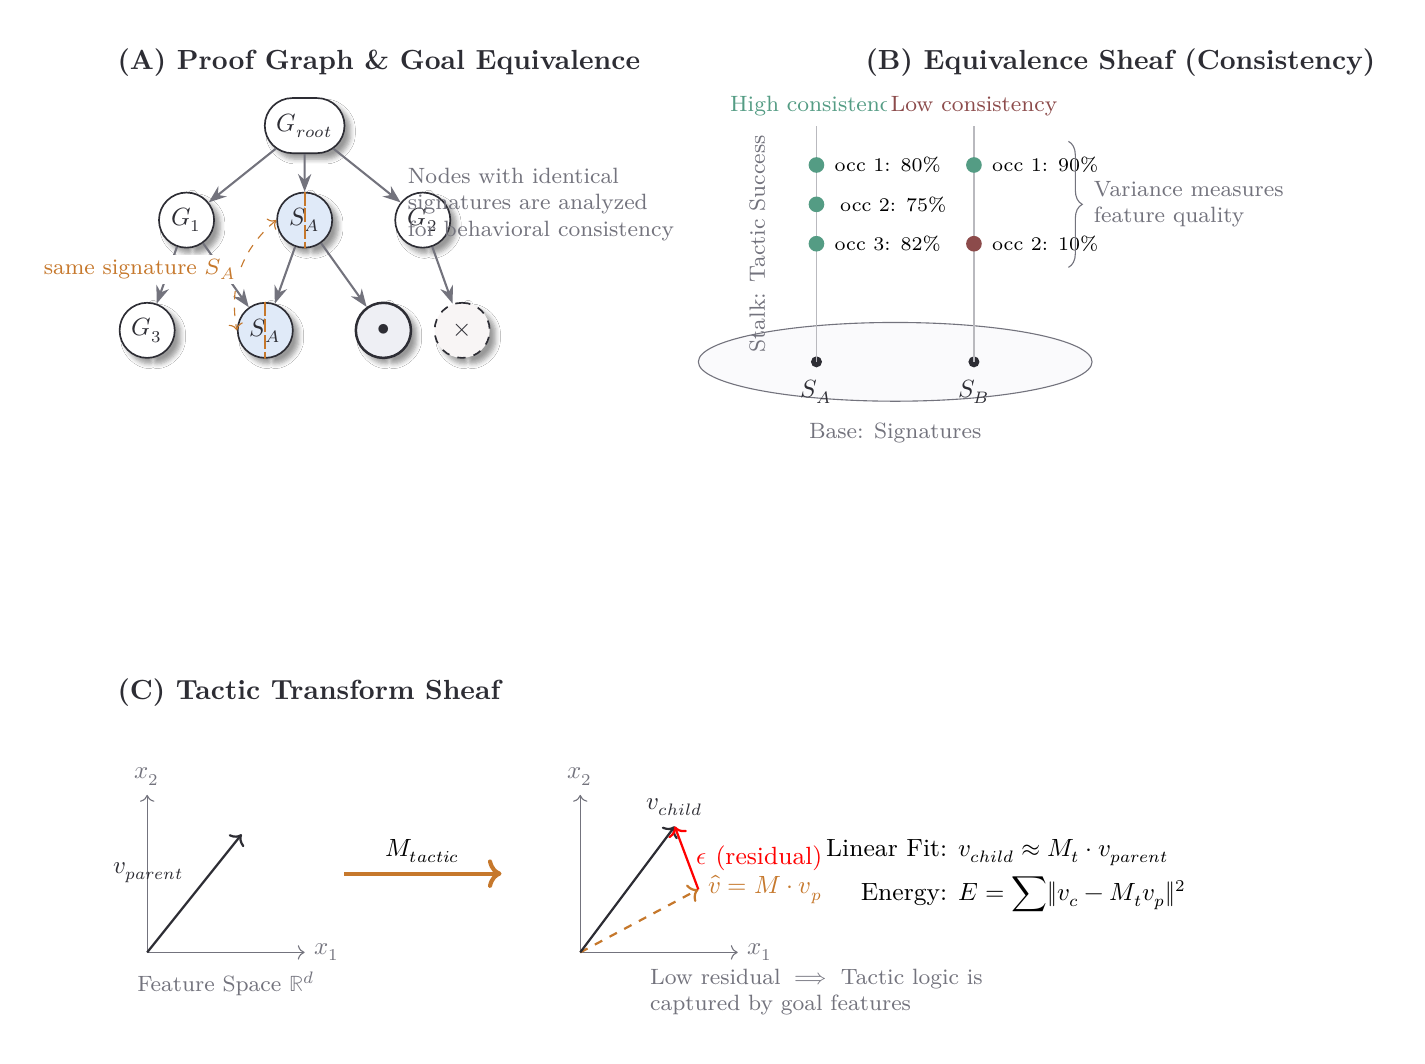
\begin{tikzpicture}[
    every node/.style={font=\small},
    show background rectangle,
    background rectangle/.style={fill=white}
]

% Panel A: Proof Graph & Goal Identification
\begin{scope}[shift={(0, 0)}]
    \node[paneltitle, anchor=south west] at (-0.5, 3.5) {(A) Proof Graph \& Goal Equivalence};
    
    % Nodes in a DAG structure
    % Root
    \node[goal, minimum width=0.8cm] (n0) at (2, 3) {$G_{root}$};
    
    % Level 1
    \node[goal, minimum width=0.8cm] (n1) at (0.5, 1.8) {$G_1$};
    \node[goal, minimum width=0.8cm, fill=basin1] (n2) at (2.0, 1.8) {$S_A$}; % Signature A occurrence 1
    \node[goal, minimum width=0.8cm] (n3) at (3.5, 1.8) {$G_2$};
    
    % Level 2
    \node[goal, minimum width=0.8cm] (n4) at (0, 0.4) {$G_3$};
    \node[goal, minimum width=0.8cm, fill=basin1] (n5) at (1.5, 0.4) {$S_A$}; % Signature A occurrence 2
    \node[terminal, minimum width=0.6cm] (n6) at (3.0, 0.4) {$\bullet$};
    \node[dead, minimum width=0.6cm] (n7) at (4.0, 0.4) {$\times$};

    % Edges
    \draw[tactic] (n0) -- (n1);
    \draw[tactic] (n0) -- (n2);
    \draw[tactic] (n0) -- (n3);
    
    \draw[tactic] (n1) -- (n4);
    \draw[tactic] (n1) -- (n5); % Path converging to same signature
    \draw[tactic] (n2) -- (n5); % Diamond? Or just tree? Let's make it a DAG
    \draw[tactic] (n2) -- (n6);
    \draw[tactic] (n3) -- (n7);

    % Annotate Signature Match
    \draw[dashed, draw=highlight, line width=0.8pt] (n2.north west) rectangle (n2.south east);
    \draw[dashed, draw=highlight, line width=0.8pt] (n5.north west) rectangle (n5.south east);
    
    \draw[<->, draw=highlight, dashed, bend right=30] (n2.west) to node[left, annotbg, text=highlight] {same signature $S_A$} (n5.west);
    
    % Label
    \node[annot, align=left] at (5.0, 2.0) {Nodes with identical\\signatures are analyzed\\for behavioral consistency};
\end{scope}

% Panel B: Equivalence Sheaf (Stalks)
\begin{scope}[shift={(9.5, 0)}]
    \node[paneltitle, anchor=south west] at (-0.5, 3.5) {(B) Equivalence Sheaf (Consistency)};
    
    % Base space (Signature)
    \draw[draw=muted, fill=flowbox] (0, 0) ellipse (2.5cm and 0.5cm);
    \node[annot, anchor=north] at (0, -0.65) {Base: Signatures};
    
    % Point S_A
    \fill[ink] (-1.0, 0) circle (2pt) node[below=0.1cm] {$S_A$};
    
    % Stalk at S_A (Fiber)
    \draw[draw=muted!50] (-1.0, 0) -- (-1.0, 3.0);
    \node[annot, rotate=90] at (-1.75, 1.5) {Stalk: Tactic Success};
    
    % Data points on stalk (Occurrences)
    % Consistent example
    \node[circle, fill=accentgreen, inner sep=2pt, label={right:\scriptsize occ 1: 80\%}] at (-1.0, 2.5) {};
    \node[circle, fill=accentgreen, inner sep=2pt, label={[xshift=2pt]right:\scriptsize occ 2: 75\%}] at (-1.0, 2.0) {};
    \node[circle, fill=accentgreen, inner sep=2pt, label={right:\scriptsize occ 3: 82\%}] at (-1.0, 1.5) {};
    
    \node[annotbg, text=accentgreen] at (-1.0, 3.25) {High consistency};

    % Point S_B (Inconsistent)
    \fill[ink] (1.0, 0) circle (2pt) node[below=0.1cm] {$S_B$};
    \draw[draw=muted!50] (1.0, 0) -- (1.0, 3.0);
    
    % Data points
    \node[circle, fill=accentgreen, inner sep=2pt, label={right:\scriptsize occ 1: 90\%}] at (1.0, 2.5) {};
    \node[circle, fill=blocked, inner sep=2pt, label={right:\scriptsize occ 2: 10\%}] at (1.0, 1.5) {};
    
    \node[annotbg, text=blocked] at (1.0, 3.25) {Low consistency};
    
    % Brace
    \draw[decorate, decoration={brace, amplitude=5pt}, draw=muted] (2.2, 2.8) -- (2.2, 1.2)
        node[midway, right=0.2cm, annot, align=left] {Variance measures\\feature quality};
\end{scope}

% Panel C: Transform Sheaf (Linear Maps)
\begin{scope}[shift={(0, -7.5)}]
    \node[paneltitle, anchor=south west] at (-0.5, 3.0) {(C) Tactic Transform Sheaf};
    
    % Parent Feature Space
    \begin{scope}[shift={(0,0)}]
        \draw[->, muted] (0,0) -- (2,0) node[right] {$x_1$};
        \draw[->, muted] (0,0) -- (0,2) node[above] {$x_2$};
        \draw[thick, ink, ->] (0,0) -- (1.2, 1.5) node[midway, above left] {$v_{parent}$};
        \node[annot] at (1.0, -0.4) {Feature Space $\mathbb{R}^d$};
    \end{scope}
    
    % Transformation Arrow
    \draw[->, line width=1.5pt, draw=highlight] (2.5, 1.0) -- (4.5, 1.0) node[midway, above] {$M_{tactic}$};
    
    % Child Feature Space
    \begin{scope}[shift={(5.5,0)}]
        \draw[->, muted] (0,0) -- (2,0) node[right] {$x_1$};
        \draw[->, muted] (0,0) -- (0,2) node[above] {$x_2$};
        
        % Predicted
        \draw[thick, highlight, ->, dashed] (0,0) -- (1.5, 0.8) node[right] {$\hat{v} = M \cdot v_p$};        
        
        % Actual
        \draw[thick, ink, ->] (0,0) -- (1.2, 1.6) node[above] {$v_{child}$};
        
        % Residual
        \draw[red, thick, ->] (1.5, 0.8) -- (1.2, 1.6) node[midway, right] {$\epsilon$ (residual)};
    \end{scope}
    
    % Matrix Equation
    \node[right] at (8.5, 1.0) {
        $\begin{aligned}
            \text{Linear Fit: } & v_{child} \approx M_t \cdot v_{parent} \\
            \text{Energy: } & E = \sum \lVert v_c - M_t v_p\rVert^2
        \end{aligned}$
    };
    
    % Interpretation
    \node[annot, align=left] at (8.5, -0.5) {Low residual $\implies$ Tactic logic is\\captured by goal features};
\end{scope}

\end{tikzpicture}
\end{document}
